\documentclass[11pt, a4 paper]{report}

\usepackage[utf8]{inputenc}
\usepackage{amsmath}
\usepackage[pdftex]{graphicx}
\usepackage{scrextend}
\usepackage{subcaption}
\usepackage{float}
\usepackage{hyperref}

\newenvironment{tabbed}{\begin{addmargin}{0.1cm}}{\end{addmargin}}
\newcommand{\sectiontitle}[1]{\begin{center} \Large\textbf{{#1}} \end{center}}
\newcommand{\sectionundertitle}[1]{\hspace{-0.5cm} \textbf{{#1}}}
\newcommand{\vsp}{\vspace{0.2cm}}

\title{FYS3150 - Project 2}
\author{Alfred Alocias Mariadason}
\date{22.09.2014}

\begin{document}
\maketitle

\sectiontitle{Introduction}
    \begin{tabbed}
        The problem at hand is to solve the Schrödinger’s equation for two electrons in a three-dimensional harmonic oscillator well. The method used for solving this is to transform(reformulate) the equation to an eigenvalue problem and then use Jacobi's method to find the eigenvalue solutions.\vsp\\
        This report focuses mainly on the implementation of Jacobi's method with a critical analysis of the results and holds some intuitive interpretation of the physics behind the results. There are also some comments on how well(bad) Jacobi's method is compared to other similar algorithms for eigenvalue problems.\vsp\\
        The language used for the implementation of Jacobi's method is C++ while the visualization(plot) is in python.\\
        Programs used in this project are new\underline prog and plotting.py. Github link for programs: \url{https://github.com/Oo1Insane1oO/project2}.
    \end{tabbed}

\sectiontitle{Theory and Algorithm}
    \sectionundertitle{The eigenvalue problem:}
        \begin{tabbed}
            As mentioned the aim of the project is to solve the Schrödinger equation. This can be archieved by transforming the equation into an eigenvalue problem and just use one of various methods to grab the eigenvalues and eigenvectors as solutions. If we assume spherical symmetry and look at one electron the equation is:
            \begin{align*}
                -\frac{\hbar^2}{2m}\bigg(\frac{1}{r^2}\frac{d}{dr}r^2\frac{d}{dr} - \frac{l(l+1)}{r^2}\bigg)R(r) + V(r)R(r) = ER(r)
            \end{align*}
            Here V is our harmonic oscillator potensial and E is the energy in three dimensions. l is just the orbital momentum(energy state) of the electron. Now we can do a substitution, $R=(1/r)u(r)$ and the equation reads:
            \begin{align*}
                -\frac{\hbar^2}{2m}\frac{d^2}{dr^2}u(r) + \bigg(V(r) + \frac{l(l+1)}{r^2}\frac{\hbar^2}{2m}\bigg)u(r) = Eu(r)
            \end{align*} 
            We know the solution at the boundaries which gives $u(0)=0$, $u(\infty)=0$. Introducing a dimensionless variable $\rho=r/\alpha$ with $\alpha$ as a variable of dimension length the equation can be further manipulated into:
            \begin{align*}
                -\frac{\hbar^2}{2m\alpha^2}\frac{d^2}{d\rho^2}u(\rho) + \bigg(V(\rho) + \frac{l(l+1)}{\rho^2}\frac{\hbar^2}{2m\alpha^2}\bigg)u(\rho) = Eu(\rho)
            \end{align*}
            We know that $V(r)=(1/2)kr^2, k=m\omega^2$, with the substitution we have $V(\rho)=(1/2)k\alpha^2\rho^2$. Inserting this into the equation and multiplying with $2m\alpha^2/\hbar^2$ gives:
            \begin{align*}
                -\frac{d^2}{d\rho^2}u(\rho) + \frac{mk}{\hbar^2}\alpha^4\rho^2u(\rho) = \frac{2m\alpha^2}{\hbar^2}Eu(\rho)
            \end{align*}
            Now we can fix $\alpha$ to work in unit lengths:
            \begin{align*}
                \frac{mk}{\hbar^2}\alpha^4 = 1 \Rightarrow \alpha = \bigg(\frac{\hbar^2}{mk}\bigg)^{1/4}
            \end{align*}
            Now we define $\lambda=(2m\alpha^2/\hbar^2)E$ and the final equation can be written as:
            \begin{align*}
                -\frac{d^2}{d\rho^2}u(\rho) + \rho^2u(\rho) = \lambda u(\rho)
            \end{align*}
            Here $\lambda$ simply represents the energy levels and $\rho$ is the distance in dimension length. The derivated part of the equation can be approximated with the standard equation for second derivative. If we do this and define $\rho_i=rho_min + ih, i=1,2\dots,n_{step}$ where $h$ is the step given as $h=(\rho_{max}-\rho_{min})/n_{step}$. The approximated equation is then:
            \begin{align*}
                -\frac{u_{i+1}-2u_i+u_{i-1}}{h^2} + \rho^2_i u_i = -\frac{u_{i+1}-2u_i+u_{i-1}}{h^2} + V_iu_i = \lambda u_i
            \end{align*}
            Here $V_i=\rho^2_i$ is the potensial. To write this into a matrix we set the diagonal elements $d_i=2/h^2 + V_i$ as the mid-diagonal and $e_i=-1/h^2$ as the lower- and upper diagonals. Now all non-diagonal elements are given by a constant are thereby equal. The equation is finally:
            \begin{align*}
                d_iu_i + e_{i-1}u_{i-1} + e_{i+1}u_{i+1} = \lambda u_i
            \end{align*}
            Here $u_i$ is the unknown and the equation can be written as a matrix eigenvalue problem with the tridiagonal matrix as follows:
            \begin{align*}
                \begin{pmatrix}
                    \frac{2}{h^2}+V_1 & -\frac{1}{h^2} & 0 & 0 & \dots & 0 & 0\\
                    -\frac{1}{h^2} & \frac{2}{h^2}+V_2 & -\frac{1}{h^2} & 0 & \dots & 0\\
                    0 & -\frac{1}{h^2} & \frac{2}{h^2}+V_3 & -\frac{1}{h^2} & 0 & \dots & 0\\
                    \dots & \dots & \dots & \dots & \dots & \dots & \dots\\
                    0 & \dots & \dots & \dots & \dots & \frac{2}{h^2}+V_{n_{step}-2} & -\frac{1}{h^2}\\
                    0 & \dots & \dots & \dots & \dots & -\frac{1}{h^2} & \frac{2}{h^2}+V_{n_{step}-1}\\
                \end{pmatrix}
            \end{align*}
            Now we can use an eigenvalue algorithm like Jacobi's method, covered in the next section, to solve this matrix.
        \end{tabbed}\vsp
    \sectionundertitle{Jacobi's method:}
    \begin{tabbed}
        Jacobi's method bases itself on transforming a tridiagonal matrix, making it converge towards a tridiagonal form with the eigenvalues along the mid-diagonal. This is archived by rotating the matrix with an angle theta. The rotation process is made by multiplying our matrix with an orthogonal transformation matrix. More specifically we have an $(n\times n)$ orthogonal transformation matrix:
        \begin{align*}
            S =
            \begin{pmatrix}
                1 & 0 & \dots & 0 & 0 & \dots & 0 & 0\\
                0 & 1 & \dots & 0 & 0 &\dots & 0 & 0\\
                \dots & \dots & \dots & \dots & \dots & \dots & 0 & \dots\\
                0 & 0 & \dots & \cos{\theta} & 0 & \dots & 0 & \sin{\theta}\\
                0 & 0 & \dots & 0 & 1 & \dots & 0 & 0\\
                \dots & \dots & \dots & \dots & \dots & \dots & 0 & \dots\\
                0 & 0 & \dots & 0 & 0 & \dots & 1 & 0\\
                0 & 0 & \dots & -\sin{\theta} & \dots & \dots & 0 & \cos{\theta}
            \end{pmatrix}
        \end{align*}
        This matrix(as mentioned above) executes a plane rotation around an angle $\theta$. We also have that $S^T=S^{-1}$. Considering this rotation the elements not 0 are given by:
        \begin{align*}
            s_{kk} &= s_{ll} = \cos{\theta}\\
            s_{kl} &= -s_{lk} = -\sin{\theta}\\
            s_{ii} &= -s_{ii} = 1\\
            i &\neq k\\
            i &\neq l
        \end{align*}
        As mentioned the rotation process is basically multiplying the transformation matrix S with our matrix. Let's call our matrix for A and the new matrix for B. The similarity transformation is then given as:
        \begin{align*}
            B = S^TAS
        \end{align*}
        The resulting algorithm is then:
        \begin{align*}
            b_{ii} &= a_{ii}\\
            b_{ik} &= a_{ik}\cos{\theta} - a_{il}\sin{\theta}\\
            b_{il} &= a_{il}\cos{\theta} + a_{ik}\sin{\theta}\\
            b_{kk} &= a_{kk}\cos^2{\theta} - 2a_{kl}\cos{\theta}\sin{\theta} + a_{ll}\sin^2{\theta}\\
            b_{ll} &= a_{ll}\cos^2{\theta} + 2a_{kl}\cos{\theta}\sin{\theta} + a_{kk}\sin^2{\theta}\\
            b_{kl} &= (a_{kk} - a_{ll})\cos{\theta}\sin{\theta} + a_{kl}(\cos^2{\theta} - \sin^2{\theta})\\
            i &\neq k, i \neq l
        \end{align*}
        The point here is to choose a $\theta$ that makes $b_{kl}$(the non-digonal matrix elements) become zero. This is archieved by defining a t as $\tan{\theta = \frac{s}{c}}$ and $\tau=\frac{a_{ll}-a_{kk}}{2a_{kl}}$ . We then obtain a quadratic equation:
        \begin{align*}
            t^2 + 2\tau t - 1 = 0 \Rightarrow t = -\tau \pm \sqrt{1+\tau^2}
        \end{align*}
        s and c is respectivly $\sin{\theta}$ and $\cos{\theta}$ and from the expression for t, $c = \frac{1}{\sqrt{1+t^2}}$ and $s=tc$. It is easy to see from the expression of c that chosing the smaller $t$ will result in a $\theta$ value which is smaller than 1, this in turn gives the angle $\theta \leq \pi/4$. This last result basically ensures that the difference between our original matrix and the rotated matrix is as small as possible.\vsp\\
        Jacobi's method is alot slower than other eigenvalue solvers. Jacobi's is also a bit unstable because one might not get zeros outside of the diagonal, that is, next iteration might change a non-diagonal element which is zero to non-zero. This means that increasing the number of iterations can actually give non-zero elements where you don't want.\vsp\\
    \end{tabbed}

\sectiontitle{Results of Jacobi's method}
    \begin{tabbed}
        Running new\textunderscore prog with an $n_{step}=280$ gives these eigenvalues(5 first):\\
        \begin{center}
        \begin{tabular}{l|l}
            $\boldsymbol{\rho_{max}=5}$ & $\boldsymbol{\rho_{max}=10}$\\ \hline
            2.999901 & 2.999604\\
            6.999508 & 6.998021\\
            10.998990 & 10.995170\\
            15.003610 & 14.991050\\ 
            19.069403 & 18.985662\\ 
        \end{tabular}
        \end{center}\vsp
        With some intuitive experimentation the lowest $n_{step}$ in order to get the lowest three eigenvalues with four leading digits is 280. This was archieved with $\rho_{max}=10$. Increasing $\rho_{max}$ beyond this only gave worse results. Decreasing it didn't yield any better results either.\vsp\\
        Number of similarity transformations:\\
        \begin{center}
            \begin{tabular}{c|c}
                $n$ & Transformations\\ \hline
                10 & 113\\
                100 & 17293\\
                150 & 39377\\
                200 & 70538\\
                280 & 139511\\
                500 & 447415 
            \end{tabular}
        \end{center}
        The only behaviour one can see here is that the number of similarity transformations needed is determined by a factor about $1.75n^2$. 
    \end{tabbed}\vsp
\newpage
    \sectionundertitle{Jacobi compared to armadillo solve:} \vsp
    \begin{tabbed}    
        The time usage for both methods:
        \begin{center}
        \begin{tabular}{l|c|c}
            $n_{step}$ & Jacobi method & Armadillo solve\\ \hline
            $10$ &$418\mu$s & $128\mu$s\\
            $100$ & $230$ms & $1$ms\\
            $150$ & $1$s & $2$ms\\
            $200$ & $3$s & $5$ms\\
            $280$ & $16$s & $11$ms\\
            $500$ & $168$s & $60$ms
        \end{tabular}
        \end{center}\vsp
        One can see here that the time usage for Jacobi's method is ridiculous compared to armadillo's solve. The conclusion here is that Jacobi's method is very(very) slow, but fairly simple to implement and aslong as we ensure $\theta \leq \pi/4$ it does give a good result. The reason behind why the method is so slow is because of the number of operations needed for the algorithm to function. We first need to do the similarity transformation, and check for the right t and on top of this the maximal off-diagonal element needs to be found. Just by looking at the program where the method is implemented it is easy to see that it is a fairly long code to chew through.
    \end{tabbed}

\sectiontitle{Two electrons in a harmonic oscillator well}
    \begin{tabbed}
        We can use the Schrodinger equation to study electrons in an oscillator well by looking at the wavefunction for the groundstate with varying $\omega_r$. Now our potensial is on form $V=\omega_r^2\rho^2+1/\rho$. The procedure for aquiring the new equation(and the new potensial form) follows the same as in the first form, but we now use the relative distance between the two electrons. The equation will have the same form as previously. Let's first look at the wavefunction as potensial over distance(potensial on y-axis and distanse $\rho$ on x-axis) for varying $\omega_r$:
        \begin{figure}[H]
            \centering
            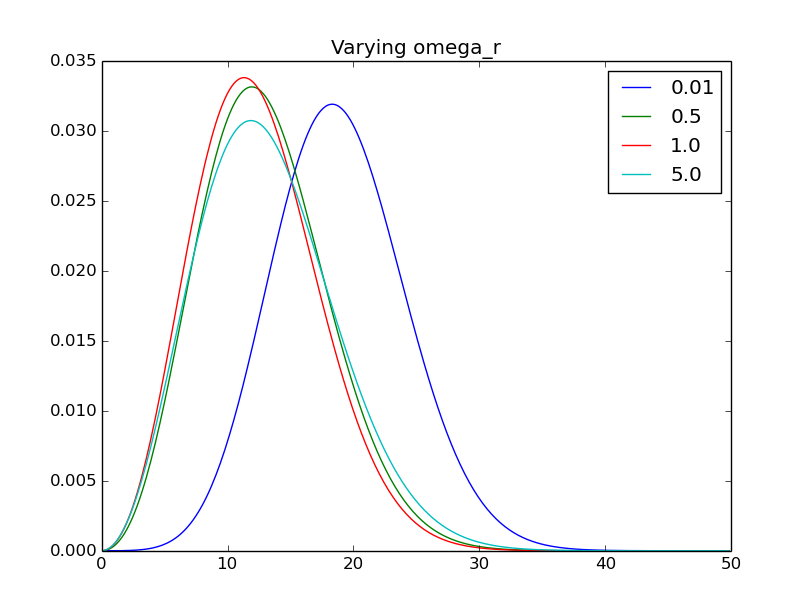
\includegraphics[scale=0.4]{vary.png}
        \end{figure}
    \end{tabbed}
        We can see here that the shape of the curve changes, an $\omega_r$ close to 1 gives a higher maximum potensial and a larger $\omega_r$ makes the potensial curves converge closer to eachother. This is a fairly logical result since $\omega_r$ is the parameter which determines the strength of the oscillator potensial. A large $\omega_r$ gives a large potensial, with other words the repulsion in the wall is large and the oscillation will ofcourse happen over a smaller distance.

\sectiontitle{Wavefunction for two electrons}
    \begin{tabbed}
    In this section we want to plot the wavefunction for two electrons. With the repulsion(Coulomb interaction) the plots look something like this:
    \end{tabbed}
    \begin{figure}[H]
        \captionsetup[subfigure]{labelformat=empty}
        \begin{subfigure}[b!]{0.6\textwidth}
            \centering
            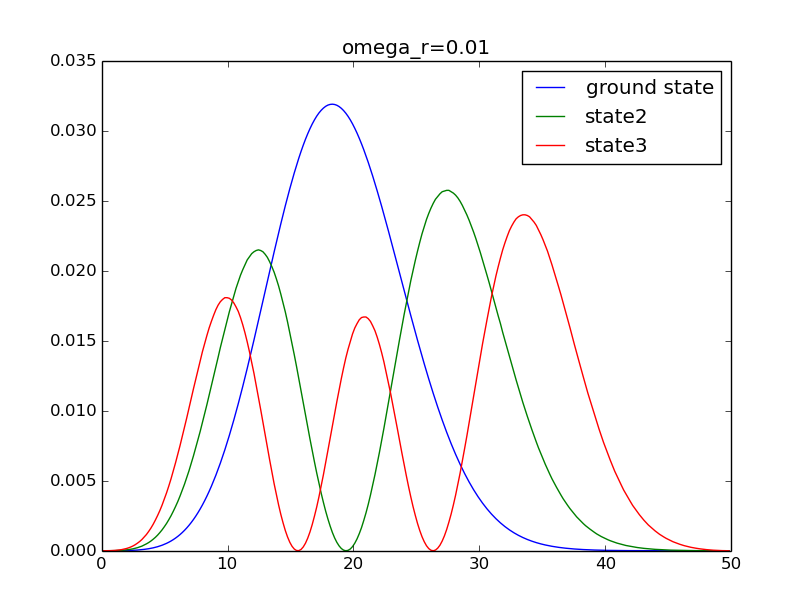
\includegraphics[width=\textwidth]{or001.png}
            \caption{$\omega_r=0.01$}
        \end{subfigure}
        \begin{subfigure}[b!]{0.6\textwidth}
            \centering
            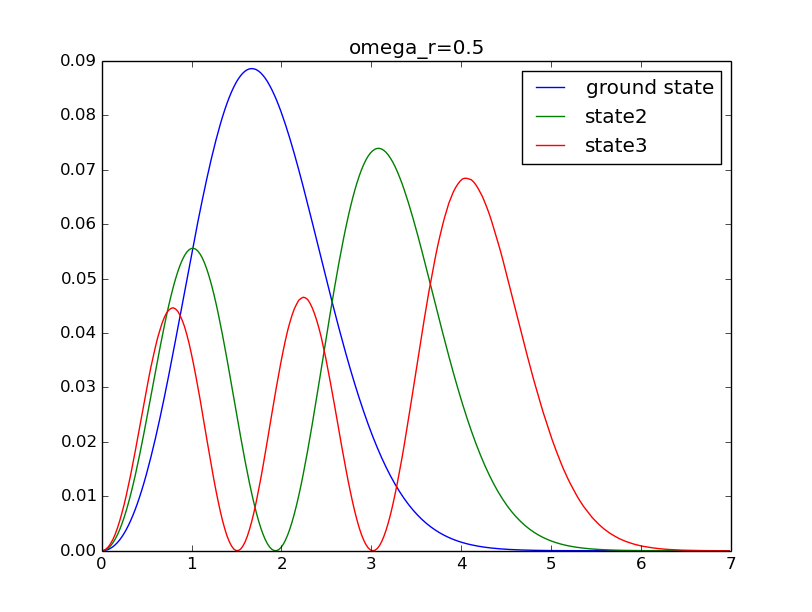
\includegraphics[width=\textwidth]{or05.png}
            \caption{$\omega_r=0.5$}
        \end{subfigure}
    \end{figure}
    \begin{figure}[H] 
        \captionsetup[subfigure]{labelformat=empty}
        \begin{subfigure}[b!]{0.6\textwidth}
            \centering
            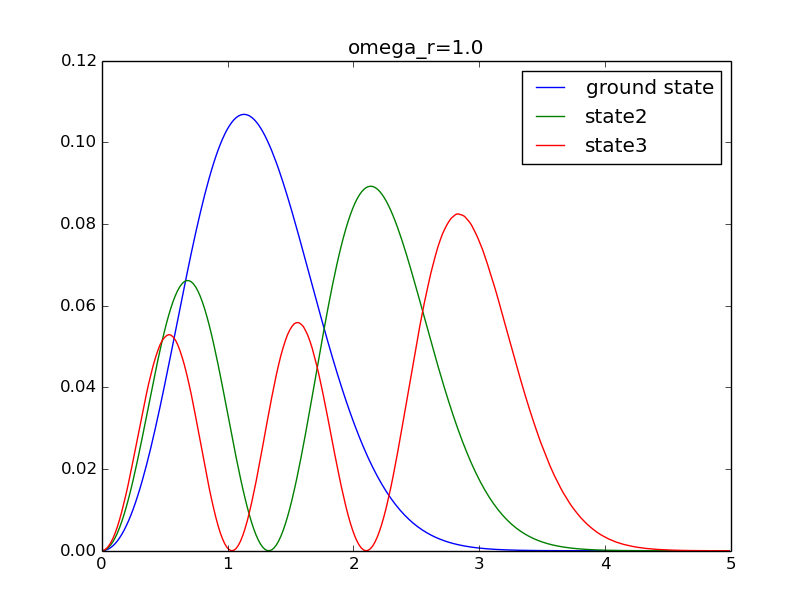
\includegraphics[width=\textwidth]{or1.png}
            \caption{$\omega_r=1.0$}
        \end{subfigure}
        \begin{subfigure}[b!]{0.6\textwidth}
            \centering
            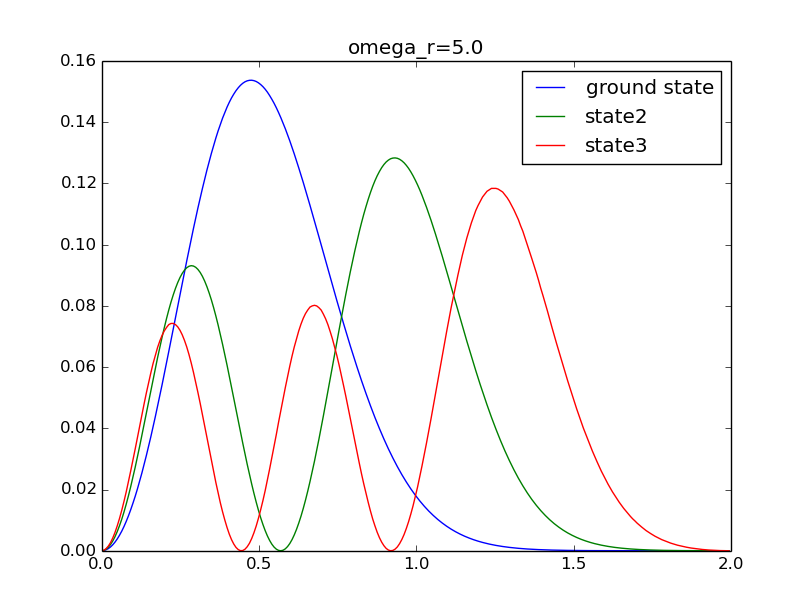
\includegraphics[width=\textwidth]{or5.png}
            \caption{$\omega_r=5.0$}
        \end{subfigure}
    \end{figure}
    \begin{tabbed}
    Note: the plots are of the probability distribution(the wavefunction squared).\vsp\\
    Increasing $\omega_r$ makes the graph shorter, which does make sense since this is our defined frequency(and also strength of potensial). So increasing the frequancy reduces the distance at which the particle travels, with other words, the maximum potensial is archieved at a shorter distance.\vsp\\
    Without the repulsion we have:
    \end{tabbed}
    \begin{figure}[H]
        \centering
        \includegraphics[scale=0.5]{nc_or001.png}
    \end{figure}
    \begin{tabbed}
        Note that this is basically the result from the results of Jacobi's method.\vsp\\
        Without any interaction the graph doesn't change for different $\omega_r$(obviously since the potensial isn't dependant on $\omega_r$ in this case). The curve also spans a much smaller distance since the potensial is only determined by the distance squared($V=\rho^2$).
    \end{tabbed}

\sectiontitle{Sources}
    \sectionundertitle{Project text:}
    \begin{tabbed}
        \url{http://www.uio.no/studier/emner/matnat/fys/FYS3150/h14/undervisningsmateriale/projects/project-2-deadline-september-22/project2_2014.pdf}\\
        The whole theory section is essentially just the text from here.\vsp\\
    \end{tabbed}
    \sectionundertitle{Lecture Notes(section 7.4 Jacobi's Method):}
    \begin{tabbed}
        \url{http://www.uio.no/studier/emner/matnat/fys/FYS3150/h14/undervisningsmateriale/Lecture%20Notes/lecture2014.pdf}
        \\
        The section on Jacobi's method is taken from here.\vsp\\
    \end{tabbed}
\end{document}
